\begin{enumerate}[label=\thesubsection.\arabic*.,ref=\thesubsection.\theenumi]

\numberwithin{equation}{enumi}
\numberwithin{figure}{enumi}


\item 
8-PSK 
Consider
\begin{align}
\textbf{y = s + n}
\end{align}

where \textbf{ s$\in$ \{$s_0$, $s_1$, $s_2$, $s_3$,$s_4$,$s_5$,$s_6$,$s_7$\}}

\begin{align}
    s_0 = 
    \begin{pmatrix}
     \sqrt{E_s} \\
     0
    \end{pmatrix}
\end{align}

\begin{align}
    s_1 = 
    \begin{pmatrix}
     \sqrt{\frac{E_s}{2}}\\
     \sqrt{\frac{E_s}{2}}
    \end{pmatrix}
\end{align}
\begin{align}
    s_2 = 
    \begin{pmatrix}
      0 \\
     \sqrt{E_s}
    \end{pmatrix}
\end{align}
\begin{align}
    s_3 = 
    \begin{pmatrix}
     -\sqrt{\frac{E_s}{2}}\\
     \sqrt{\frac{E_s}{2}}
    \end{pmatrix}
\end{align}
\begin{align}
    s_4 = 
    \begin{pmatrix}
     -\sqrt{E_s} \\
     0
    \end{pmatrix}
\end{align}
\begin{align}
    s_5 = 
    \begin{pmatrix}
     -\sqrt{\frac{E_s}{2}}\\
     -\sqrt{\frac{E_s}{2}}
    \end{pmatrix}
\end{align}
\begin{align}
    s_6 = 
    \begin{pmatrix}
     0\\
     -\sqrt{E_s}
    \end{pmatrix}
\end{align}
\begin{align}
    s_7 = 
    \begin{pmatrix}
     \sqrt{\frac{E_s}{2}}\\
     -\sqrt{\frac{E_s}{2}}
    \end{pmatrix}
\end{align}

\begin{figure}[!ht]
                \resizebox{\columnwidth}{!}{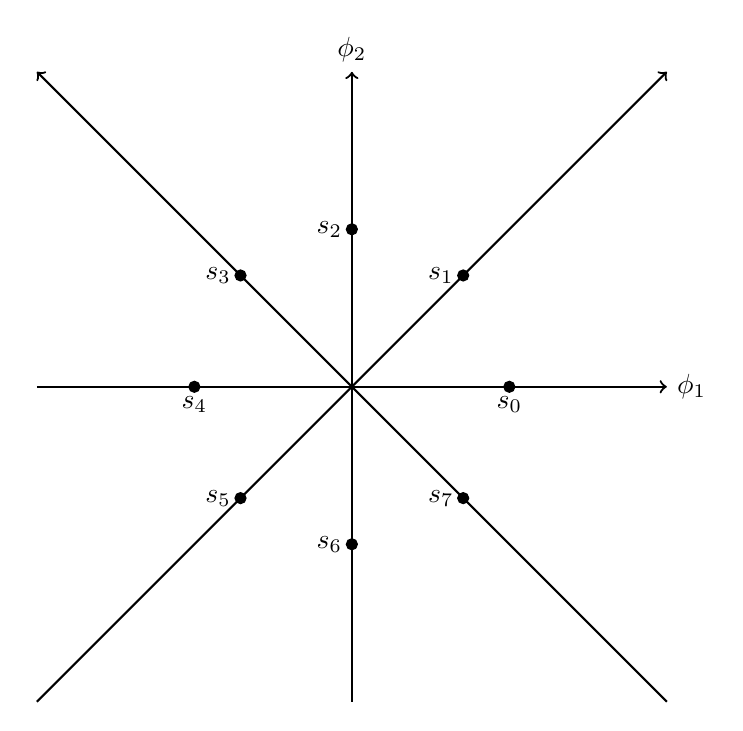
\begin{tikzpicture}

\draw[->,thick] (-4,0)--(4,0) node[right]{$\phi_1$};
\draw[->,thick] (0,-4)--(0,4) node[above]{$\phi_2$};
\draw[->,thick] (-4,-4)--(4,4) node[right]{};
\draw[->,thick] (4,-4)--(-4,4) node[above]{};

\filldraw[black] (2,0) circle (2pt) node[below] {$s_0$} ;
\filldraw[black] (1.414,1.414) circle (2pt) node[left] {$s_1$} ;
\filldraw[black] (0,2) circle (2pt) node[left] {$s_2$} ;
\filldraw[black] (-1.414,1.414) circle (2pt) node[left] {$s_3$} ;
\filldraw[black] (-2,0) circle (2pt) node[below] {$s_4$} ;
\filldraw[black] (-1.414,-1.414) circle (2pt) node[left] {$s_5$} ;
\filldraw[black] (0,-2) circle (2pt) node[left] {$s_6$} ;
\filldraw[black] (1.414,-1.414) circle (2pt) node[left] {$s_7$} ;


\end{tikzpicture}
}
\label{fig:ee18btech11012_fig1}
\caption{Constellation diagram}
\end{figure}


\item Encoding

$s_0$ denote bits 000, $s_1$ denote bits 001, $s_2$ denote bits 011,$s_3$ denote bits 010,$s_4$ denote bits 110,$s_5$ denote bits 111,$s_6$ denote bits 101,$s_7$ denote bits 100.
\begin{figure}[!ht]
                \resizebox{\columnwidth}{!}{\input{./figs/ee18btech11012_1.tex}}
\label{fig:ee18btech11012_fig2}
\caption{Gray coding}
\end{figure}

\item Decoding



\begin{figure}[!ht]

                \resizebox{\columnwidth}{!}{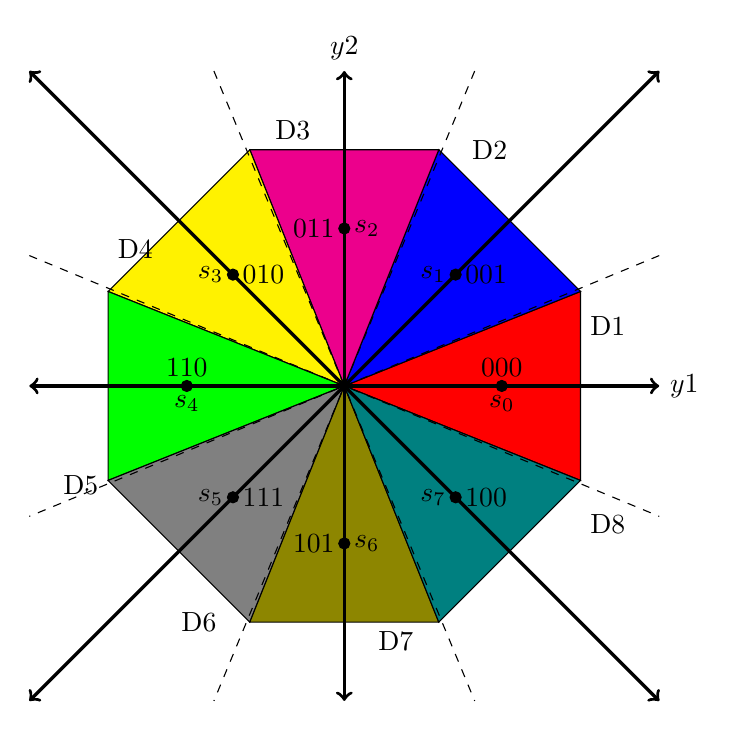
\begin{tikzpicture}
\draw[fill=red]  (0,0) -- (3,1.2) -- (3,-1.2) -- (0,0) -- cycle;
\draw[fill=blue]  (0,0) -- (1.2,3) -- (3,1.2) -- (0,0) -- cycle;
\draw[fill=magenta!100]  (0,0) -- (-1.2,3) -- (1.2,3) -- (0,0) -- cycle;
\draw[fill=yellow]  (0,0) -- (-1.2,3) -- (-3,1.2) -- (0,0) -- cycle;
\draw[fill=green]  (0,0) -- (-3,1.2) -- (-3,-1.2) -- (0,0) -- cycle;
\draw[fill=gray]  (0,0) -- (-3,-1.2) -- (-1.2,-3) -- (0,0) -- cycle;
\draw[fill=olive]  (0,0) -- (-1.2,-3) -- (1.2,-3) -- (0,0) -- cycle;
\draw[fill=teal]  (0,0) -- (1.2,-3) -- (3,-1.2) -- (0,0) -- cycle;
\draw[<->,very thick] (-4,0)--(4,0) node[right]{$y1$};
\draw[<->,very thick] (0,-4)--(0,4) node[above]{$y2$};
\draw[dashed] (4,1.656)--(-4,-1.656);
\draw[dashed] (1.656,4)--(-1.656,-4);
\draw[dashed] (-1.656,4)--(1.656,-4);
\draw[dashed] (-4,1.656)--(4,-1.656);
\draw[<->,very thick](-4,-4)--(4,4);
\draw[<->,very thick](-4,4)--(4,-4);

\filldraw[black] (2,0) circle (2pt) node[below] {$s_0$} node[above] {000};
\filldraw[black] (1.414,1.414) circle (2pt) node[left] {$s_1$} node[right] {001};
\filldraw[black] (0,2) circle (2pt) node[right] {$s_2$} node[left] {011};
\filldraw[black] (-1.414,1.414) circle (2pt) node[left] {$s_3$} node [right] {010};
\filldraw[black] (-2,0) circle (2pt) node[below] {$s_4$} node[above] {110};
\filldraw[black] (-1.414,-1.414) circle (2pt) node[left] {$s_5$} node[right] {111};
\filldraw[black] (0,-2) circle (2pt) node[right] {$s_6$} node[left] {101};
\filldraw[black] (1.414,-1.414) circle (2pt) node[left] {$s_7$} node [right] {100};

\foreach \coordinate/\label/\pos in {{(3,1)/D1/below right},{(1.5,3)/D2/right},{(-1,3)/D3/above right},{(-3,1.5)/D4/above right},{(-3,-1.5)/D5/above left},{(-1.5,-3)/D6/left},{(1,-3)/D7/below left},{(3,-2)/D8/above right}} \node[\pos] at \coordinate {\label};

\end{tikzpicture}
}

\label{fig:ee18btech11012_fig3}
\caption{decision regions}
	
\end{figure}

\textbf{\underline{Minimum distance Criterion}:}
\begin{align}
    \hat{s} = min \norm{\textbf{y} - \textbf{s}}
    \label{eq:ee18btech11012_eq1}
\end{align}
where \textbf{s} \in {$s_{0}$,$s_{1}$,$s_{2}$,.....$s_{M}$}\\
From eq.\ref{eq:ee18btech11012_eq1},\textbf{$s_{0}$} is chosen if
\begin{align}
    \norm{\textbf{y}-\textbf{$s_{0}$}}^2 < \norm{\textbf{y}-\textbf{$s_{1}$}}^2
\end{align}
\begin{align}
    \norm{\textbf{y}-\textbf{$s_{0}$}}^2 < \norm{\textbf{y}-\textbf{$s_{2}$}}^2
\end{align}
\begin{align}
    \norm{\textbf{y}-\textbf{$s_{0}$}}^2 < \norm{\textbf{y}-\textbf{$s_{3}$}}^2
\end{align}
\begin{align}
    \norm{\textbf{y}-\textbf{$s_{0}$}}^2 < \norm{\textbf{y}-\textbf{$s_{4}$}}^2
\end{align}
\begin{align}
    \norm{\textbf{y}-\textbf{$s_{0}$}}^2 < \norm{\textbf{y}-\textbf{$s_{5}$}}^2
\end{align}
\begin{align}
    \norm{\textbf{y}-\textbf{$s_{0}$}}^2 < \norm{\textbf{y}-\textbf{$s_{6}$}}^2
\end{align}
\begin{align}
    \norm{\textbf{y}-\textbf{$s_{0}$}}^2 < \norm{\textbf{y}-\textbf{$s_{7}$}}^2
\end{align}
Since $\norm{s_{i}}^2$ = $E_{s}$,the above conditions can be simplified to obtain the region
\begin{align}
    (s_{0}-s_{1})^Ty>0
\end{align}
\begin{align}
    (s_{0}-s_{2})^Ty>0
\end{align}
\begin{align}
    (s_{0}-s_{3})^Ty>0
\end{align}
\begin{align}
    (s_{0}-s_{4})^Ty>0
\end{align}
\begin{align}
    (s_{0}-s_{5})^Ty>0
\end{align}
\begin{align}
    (s_{0}-s_{6})^Ty>0
\end{align}
\begin{align}
    (s_{0}-s_{7})^Ty>0
\end{align}
Substituting the values of $s_{0}$,$s_{1}$,....$s_{7}$ in the above and eliminating $\sqrt{E_{s}}$,,the desired region is
\begin{align}
    \myvec{(1-\frac{1}{\sqrt{2}})\\\frac{-1}{\sqrt{2}}}^T\myvec{y_{1}\\y_{2}} > 0
\end{align}
\begin{align}
    \myvec{1\\-1}^T\myvec{y_{1}\\y_{2}} > 0
\end{align}
\begin{align}
    \myvec{(1+\frac{1}{\sqrt{2}})\\\frac{-1}{\sqrt{2}}}^T\myvec{y_{1}\\y_{2}} > 0
\end{align}
\begin{align}
    \myvec{1\\0}^T\myvec{y_{1}\\y_{2}} > 0
\end{align}
\begin{align}
    \myvec{(1+\frac{1}{\sqrt{2}})\\\frac{1}{\sqrt{2}}}^T\myvec{y_{1}\\y_{2}} > 0
\end{align}
\begin{align}
    \myvec{1\\1}^T\myvec{y_{1}\\y_{2}} > 0
\end{align}
\begin{align}
    \myvec{(1-\frac{1}{\sqrt{2}})\\\frac{1}{\sqrt{2}}}^T\myvec{y_{1}\\y_{2}} > 0
\end{align}
yielding $y_2+(\sqrt{2}-1)y_1>0$, $y_2-(\sqrt{2}-1)y_1<0$.\\i.e.,Red region(D1) is detected at the receiver.
\\


Similarly for all symbols their decision region and their respective inequalities are given below in the table shown.
\begin{figure}[!ht]
                \resizebox{\columnwidth}{!}{\input{./figs/ee18btech11012_2.tex}}
\label{fig:ee18btech11012_fig4}
\caption{Decision regions and their inequalities}
\end{figure}



\item The following code has simulation of 8PSK.
\begin{lstlisting}
 codes/ee18btech11012.py
\end{lstlisting}
\end{enumerate}
